\section{Introducción}

\subsection{Contexto}
En las últimas décadas, la revolución tecnológica ha posibilitado que el desarrollo e implementación de satélites en \gls{LEO} a una escala sin precedentes \cite{ref1}. Entre estos, los CubeSats han surgido como una solución eficiente y versátil para una amplia gama de aplicaciones. Los CubeSats son nanosatélites que se ajustan a un estándar que especifica sus dimensiones y diseño. Estos vienen en varios tamaños, siendo los más comunes 1U, 3U, 6U y 12U. La “U” en estas designaciones de tamaño significa “unidad” y se refiere al tamaño de un CubeSat en términos del número de unidades cúbicas de 10 x 10 x 11.35 [cm\textsuperscript{3}] que lo componen \cite{ref2}. Se puede observar la relevancia de este tipo de satélites según la cantidad de lanzamientos que se han realizado a través de los años y de los confirmados a futuro en la Figura~\ref{fig:nanosats}.

\begin{figure}[h]
	\centering    
	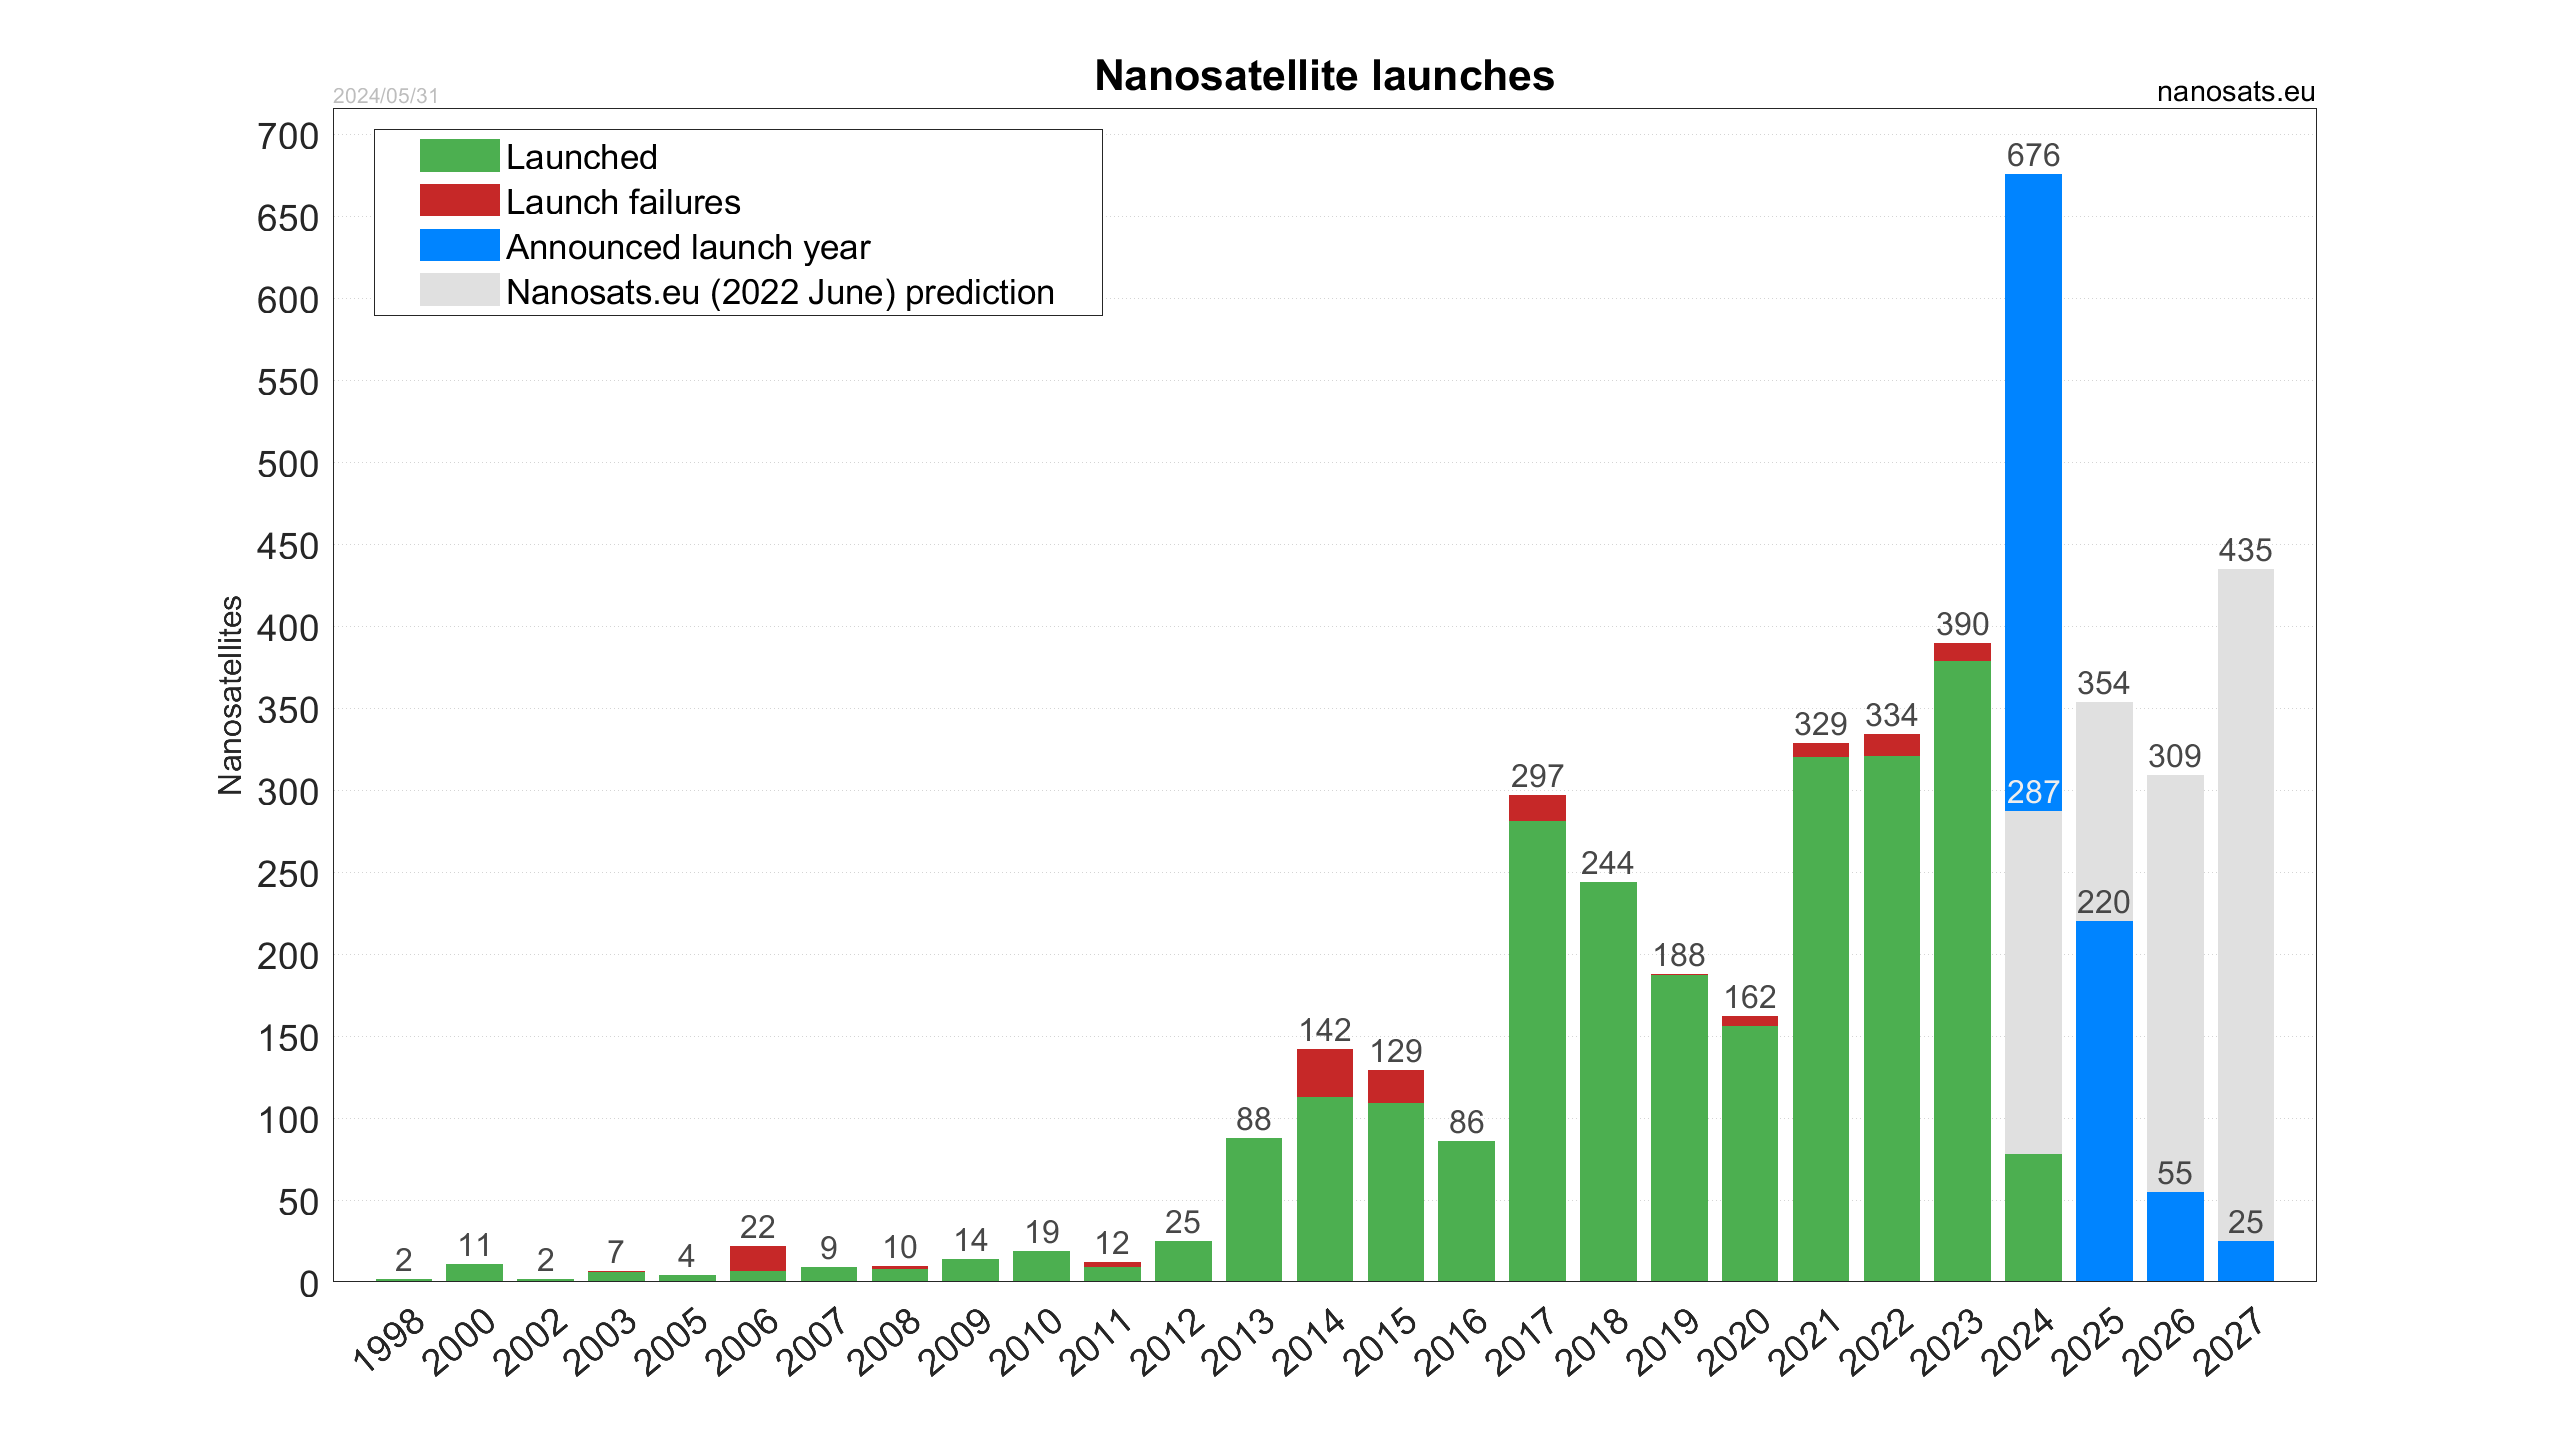
\includegraphics[width=1\textwidth]{Nanosats_years_2024-05-31_large.png}
	\caption{Cantidad de nanosatélites lanzados a través de los años \cite{ref1}.}.
	\label{fig:nanosats}
\end{figure}

Dentro de estos nanosatélites, una aplicación con gran porcentaje de ocurrencia en el ámbito comercial está enfocado en la observación terrestre mediante la utilización de cargas útiles ópticas \cite{ref3}. Esta aplicación consiste en la captura de imágenes de la superficie terrestre utilizando sensores que detectan distintas partes del espectro electromagnético. Estos sensores ópticos funcionan al detectar la luz reflejada (generalmente luz infrarroja cercano o visible) en la superficie de la Tierra \cite{ref4}.

Para llevar a cabo este tipo de misión, se requiere de una capacidad de apuntamiento con el fin de cumplir el objetivo de capturar imágenes con la calidad y resolución requeridas. El concepto de apuntamiento se define como la capacidad del satélite para ajustar su actitud, logrando un cambio de orientación hacia un objetivo deseado \cite{ref5}. 

Para determinar y/o caracterizar la capacidad de apuntamiento, es necesario medir y evaluar su desempeño a través de los \gls{MoP} relevantes para las misiones de observación terrestre. En estudios anteriores \cite{ref5, ref6, ref7, ref8} , se proporciona una definición cualitativa de los siguientes MoP de apuntamiento, los cuales están condicionados por la calidad del hardware y software (algoritmos de estimación y/o determinación de actitud) correspondientes al \gls{ADCS}:

\begin{itemize}
	\item Exactitud de apuntamiento \cite{ref5,ref7}: Definido como el error absoluto entre la orientación requerida.
	\item Drift \cite{ref5}: Se refiere a cuánto puede desviarse un vehículo con el tiempo. Este parámetro es crucial cuando se necesita mantener una dirección específica y se deben hacer correcciones solo ocasionalmente para evitar que el vehículo se desvíe significativamente de su curso deseado. Representado mediante ángulos por hora [°/hr].
	\item Jitter \cite{ref9,ref10}: Se representa como las vibraciones mecánicas de alta frecuencia que provocan una visualización difuminada en la cámara y se cuantifica como la \gls{PSD} del filtro pasa alto de la respuesta a la estabilización del satélite.
	\item Agilidad \cite{ref11}: Se describe como el tiempo de asentamiento con el cual se estabiliza el CubeSat a la orientación deseada, representada en segundos. Generalmente mediante una banda de asentamiento del 5\%.
\end{itemize}

En conjunto con los parámetros de apuntamiento, es crucial considerar los System Engineering (SE) envelopes específicos para el tipo de misión y satélite en uso. Estos SE envelopes son restricciones técnicas y operativas que deben ser consideradas durante las fases de diseño, desarrollo y operación del CubeSat. Los parámetros clave de estos envelopes incluyen la potencia eléctrica, la masa, el tamaño/volumen y el costo.

Los SE envelopes se definen principalmente en función de la carga útil, que es el punto de partida para el diseño y desarrollo de los demás subsistemas del satélite, especialmente el \gls{ADCS}, que es fundamental para el apuntamiento del satélite \cite{ref8}.

Dado que los CubeSats tienen restricciones de masa y volumen (de acuerdo con el estándar de unidades), y se busca minimizar costos al limitar el costo de componentes y reducir la superficie de paneles solares (y por ende la potencia y energía disponible), es necesario establecer requerimientos específicos para los SE envelopes del satélite y los parámetros de apuntamiento. Esto se debe hacer de acuerdo con la complejidad de la misión de observación terrestre, para encontrar un equilibrio óptimo entre estos aspectos y satisfacer las necesidades de la misión.

Por lo tanto, es esencial definir claramente los aspectos de la misión, tales como la dinámica orbital (incluyendo los parámetros orbitales y las perturbaciones en órbita baja (LEO)) y la geometría del satélite, así como las limitaciones y capacidades del \gls{ADCS}. Esto permitirá conocer el costo asociado a la misión y su desempeño en términos de apuntamiento. La Figura~\ref{fig:bloques01} presenta un diagrama que ilustra esta interacción, mostrando una visualización gráfica de los parámetros de costo y rendimiento.

\begin{figure}[h]
	\centering    
	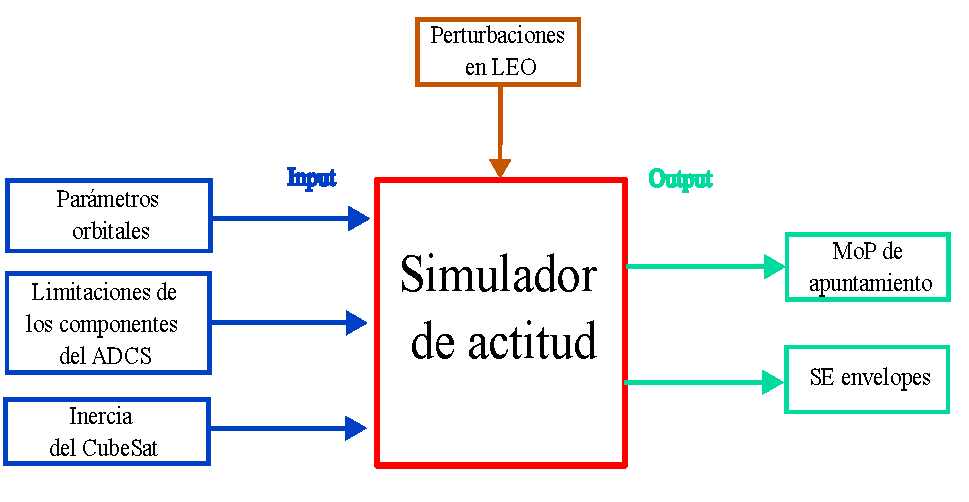
\includegraphics[width=0.9\textwidth]{diagrama memoria1234.pdf}
	\caption{Representación gráfica de la relación entre aspectos de la misión respecto a costo y rendimiento (Elaboración propia).}
	\label{fig:bloques01}
\end{figure}

Existen estudios que simulan diversos aspectos del \gls{ADCS}, incluyendo los componentes físicos \cite{ref12}, algoritmos de determinación de actitud \cite{ref13} y controladores \cite{ref14}. En estos trabajos, se analizan y comparan los diferentes elementos del \gls{ADCS} para identificar cuáles ofrecen mejores rendimientos, con un enfoque particular en el budget de potencia, que es uno de los factores más relevantes. Además, también se han realizado estudios en los que se simula el \gls{ADCS} completo de un CubeSat, especificando tanto su diseño como los resultados de su rendimiento \cite{ref15,ref16,ref17}.

Por otro lado, en \cite{ref18} y \cite{ref19} se presentan herramientas y simuladores capaces de implementar la dinámica orbital y de actitud, proporcionando una interfaz gráfica que visualiza los movimientos traslacionales y rotacionales, así como los modelos de perturbación correspondientes. Estas herramientas permiten cuantificar algunos de los Measures of Performance (MoP) de apuntamiento y evaluar los costos en función de los SE envelopes. La herramienta mencionada en \cite{ref18}, llamada Spacecraft Control Toolbox, está dividida en tres secciones según los requerimientos de las misiones. Tiene la capacidad de generar resultados relacionados con la dinámica rotacional del satélite, incluye una interfaz gráfica y, en su versión económica, estima el consumo de energía. En sus versiones académicas o profesionales, permite además recuperar errores de apuntamiento y modelar sensores y actuadores.

Además, en \cite{ref19} se presentan herramientas y plantillas disponibles en el Aerospace Blockset de MATLAB, que permiten modelar un CubeSat siguiendo especificaciones del satélite y de la órbita, y realizar simulaciones utilizando la herramienta Simulink Animation 3D para visualizar los resultados.

También existen herramientas como Valispace, cuyo propósito es principalmente el análisis de budgets de ingeniería. Un ejemplo común de su uso se describe en \cite{ref20}. Este tipo de software ofrece una visión integral del análisis de satélites, abarcando costos temporales, monetarios y de potencia, al utilizar funciones que integran los requisitos de los subsistemas involucrados.

Finalmente, existe un entorno de simulacion gratuito de la universidad de Colorado para sistemas de naves espaciales. Esta es una herramienta muy utilizada en la investigación académica y en proyectos relacionados con la simulación de dinámicas y control de vehículos espaciales de alta dificultad de uso, al combinar distintos topicos y lenguajes de programación en su arquitectura \cite{ref36}.

Teniendo esto en cuenta, el simulador propuesto se perfila como una herramienta valiosa para el análisis del \gls{ADCS} de un CubeSat. Al proporcionar la información adecuada del satélite,su órbita y el análisis especifico requerido, el simulador permitirá obtener tanto el rendimiento como el costo asociado al apuntamiento. Además, contribuirá al desarrollo tecnológico de CubeSats de manera simple y eficiente, utilizando componentes basados en CubeSats comerciales en la actualidad, todo dentro de un entorno de programación de libre acceso como Python. Asimismo, el simulador será capaz de ofrecer las características del \gls{ADCS} necesarias para alcanzar un rendimiento o costo específico, según los parámetros definidos por el usuario. Un resumen de lo que se busca una vez implementado la suite de simulacion de la Figura~\ref{fig:bloques01}, se representa en la Figura~\ref{fig:bloques02}.

\begin{figure}[h]
	\centering    
	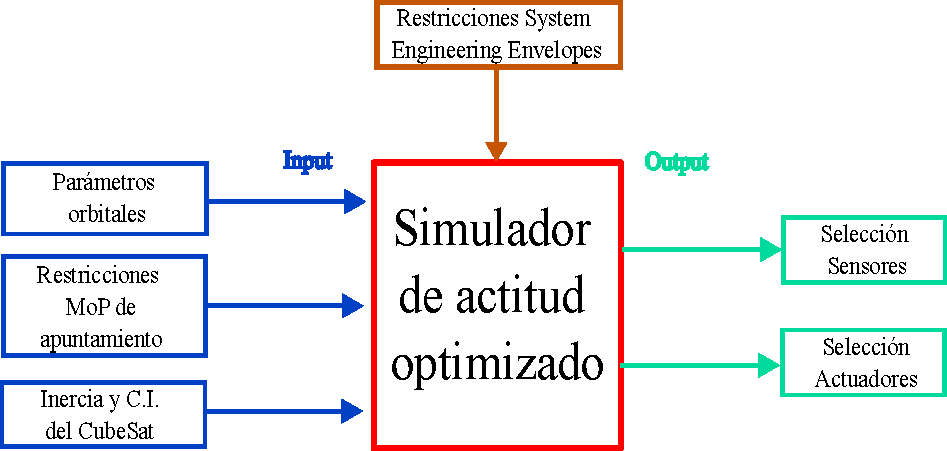
\includegraphics[width=0.9\textwidth]{bloque02.pdf}
	\caption{Solución propuesta para la suite de simulación optimizada (Elaboración propia).}
	\label{fig:bloques02}
\end{figure}

\subsection{Hipótesis}
Se postula que el diseño e implementación de una suite de simulación que modele el ambiente espacial y el \gls{ADCS}, en conjunto con un algoritmo capaz de optimizar los parámetros de rendimiento y los SE envelopes, mejorará la eficacia operativa de las misiones CubeSat al seleccionar el subconjunto óptimo de componentes físicos necesarios.

\subsection{Objetivos}
\textit{\underline{Objetivo General:}} Diseñar e implementar una suite de simulación que modele el ambiente espacial y el \gls{ADCS} de un CubeSat comercial en órbitas bajas de observación terrestre, capaz de optimizar el rendimiento (mediante los MoP de apuntamiento) y/o el costo (considerando los SE envelopes) definidos por el usuario, con el fin de seleccionar los componentes físicos del \gls{ADCS} necesarios para la misión.

\textit{\underline{Objetivos Especificos:}}

\begin{itemize}
	\item OE1: Desarrollar un marco teórico robusto sobre el modelamiento del ambiente espacial y del \gls{ADCS} de un CubeSat, enfocado en aplicaciones de observación terrestre, basadas en referencias publicadas después del año 2010.
	\item OE2: Desarrollar un modelo de ambiente espacial que permita calcular los vectores de posición y velocidad del CubeSat, junto con un modelo de actitud que incluya al menos dos sensores y dos actuadores del \gls{ADCS}.
	\item OE3:Implementar un algoritmo de estimación para el modelo dinámico del CubeSat con un margen de error inferior al 5\%.
	\item OE4: Diseñar al menos un  controlador que permita control de actitud en función de los actuadores implementados en la suite de simulación.
	\item OE5: Seleccionar e implementar un algoritmo de optimización no lineal capaz de optimizar los MoP de apuntamiento en función de los SE envelopes en la suite de simulación.
	\item OE6: Verificación cuantitativa de la suite de optimización utilizando datos empíricos del SUCHAI-3 en base a los MoP de apuntamiento obtenidos y los SE envelopes de sus componentes físicos actuales.
\end{itemize}




\subsection{Metodología}

OE1: Desarrollar el marco teórico relacionado con el \gls{ADCS} y el ambiente espacial en el simulador mediante la revisión de trabajos previos. Se recopilará información de artículos y estudios sobre la determinación y control de actitud en CubeSats, junto con el estado del arte y las especificaciones técnicas de componentes disponibles en sitios web de fabricantes, para verificar la correcta implementación de los modelos y su similitud con estudios anteriores.

OE2: Implementar el propagador SGP4 para calcular los vectores de posición y velocidad del CubeSat, teniendo en cuenta las perturbaciones orbitales en órbitas bajas. En cuanto a los modelos dinámicos de actitud, se simularán las fuerzas magnéticas y el vector solar para representar el comportamiento de sensores como el magnetómetro y el sensor solar. Los actuadores considerados en los modelos serán el magnetorquer y la rueda de reacción en los ejes del CubeSat.

OE3: Estimar los cuaterniones y las velocidades angulares del CubeSat utilizando un filtro de Kalman extendido. Este filtro será aplicado al modelo dinámico lineal discreto, integrando el magnetorquer y las ruedas de reacción. Se emplearán las mediciones simuladas de los sensores para validar las estimaciones y se evaluará la precisión de las mismas mediante el cálculo del error cuadrático medio (MSE).

OE4: Diseñar un controlador PD o LQR dentro de la suite de simulación. Una vez implementados ambos controladores, se seleccionará el de mejor rendimiento en función de los MoP de apuntamiento bajo las mismas condiciones de simulación.

OE5: Realizar una revisión de optimizadores no lineales convexos y no convexos disponibles en Python, con el objetivo de encontrar una solución óptima que maximice el rendimiento y minimice el costo en función de las entradas y requisitos del usuario. Se evaluarán herramientas como scipy.optimize y pyomo para determinar el optimizador más adecuado.

OE6: Verificar la suite de simulación utilizando datos empíricos del SUCHAI-3. Se compararán los resultados de la simulación con los parámetros reales de rendimiento de los componentes físicos y se evaluará la proximidad de los resultados obtenidos por la suite de optimización con los datos reales, determinando el conjunto óptimo de sensores y actuadores.

\subsection{Carta Gantt}                                                                                                                                                                                                               
El proyecto sigue una estructura definida contenida en la carta Gantt mostrada en el Anexo \ref{ap:Z1}. El resumen en base a los entregables se muestra a continuación en la Tabla~\ref{tab:cron}

\begin{table}[H]
	\centering
	\caption{Cronograma de hitos y avances}
	\label{tab:cron}
	\begin{tabular}{|p{4cm}|p{3.8cm}|p{4cm}|p{4cm}|}
		\hline
		\textbf{Resultado} & \textbf{Objetivos específicos asociados} & \textbf{Hito de avance} & \textbf{Fecha de entrega} \\ 
		\hline
		Finalización de la suite de simulación & OE1, OE2, OE3, OE4 & Avance I: Presentación & Semana 19 (29-02 de agosto de 2024) \\ 
		\hline
		Implementación de la optimización de parámetros en la suite de simulación & OE5 & Avance II: Informe de avance & Semana 31 (21-27 de octubre de 2024) \\ 
		\hline
		Verificación de la suite de optimización y Redacción de artículo científico & OE6 & Avance III: Entrega con manuscrito de artículo científico & Semana 37 (02-07 de diciembre de 2024) \\ 
		\hline
		Entrega final & - & Final: Presentación e informe final & Semana 41 (30 diciembre 2024-03 de enero 2025) \\ 
		\hline
	\end{tabular}
\end{table}

